\chapter{Vorüberlegungen}
Zu Beginn der Studienarbeit mussten einige Vorüberlegungen getätigt werden:
\begin{itemize}
  \item Es musste ein Datenmodell erstellt werden, welches die Struktur der Datenbank beschreibt.
  \item Es mussten alle zu der Zeit bekannten Aufgaben festgehalten werden, um sich einen Überblick über den Funktionsumfang und Arbeitsaufwand zu verschaffen.
\end{itemize}
Aus den so erhaltenen Aufgaben und den Funktionalitäten, die das Projekt am Ende bieten sollte, sollte ein Konzept zum Design einer passenden Oberfläche erstellt werden. 

\section{Datenmodell}
Das Datenmodell wurde früh entwickelt und sollte als Grundlage dienen, um die Datenstruktur der Datenbank implementieren. 
Dabei ist es wichtig Zeit in das Datenmodell zu investieren, da das Datenmodell als fundamentale Grundlage dient und große Änderungen daran später zeitaufwändige Folgen haben würden.
Dabei wurde ein eine relationale Datenbank gewählt und versucht, das Datenmodell nach den Prinzipien der Theorie der realtionalen Datenbanken aufzubauen.
Dementsprechend wurde die Tabellenstruktur in dritter Normalform aufgebaut.\\
Im Verlauf der Studienarbeit mussten dennoch Änderungen am Datenmodell vorgenommen werden, jedoch waren diese nur kleine Änderungen, wie z.B. das Hinzufügen einer Spalte innerhalb einer Tabelle.
Dies lässt den Schluss zu, dass die zu Beginn investierte Zeit in das Datenmodell und die Gespräche und Diskussionen zu Beginn hierzu sinnvoll investierte Zeit waren.

\begin{landscape}
\begin{figure}
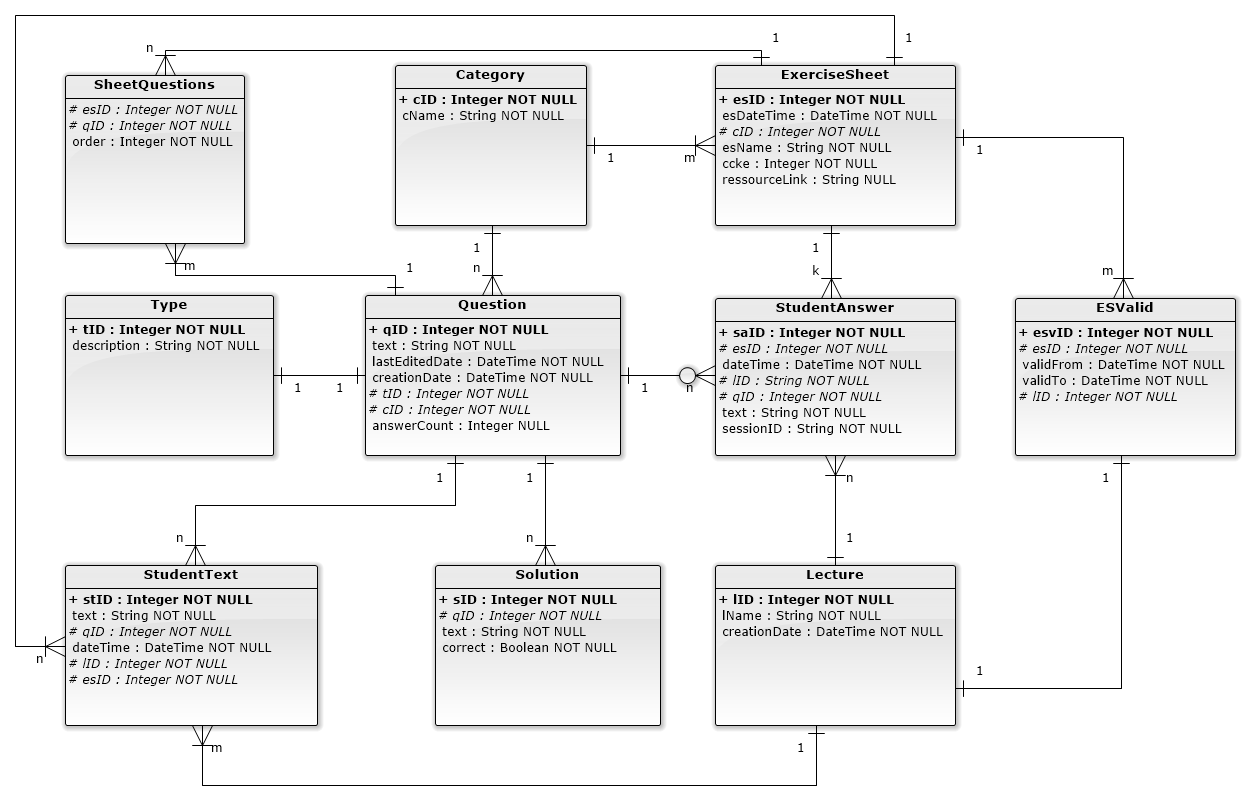
\includegraphics[height=37em]{images/Entityrelationshipdiagram.png}
\end{figure}
\end{landscape}

\section{Funktionsumfang}
Der letztendliche Funktionsumfang war zu Beginn des Projektes zwar grob klar, wie in Projekten in Unternehmen war es jedoch auch so, dass sich der Kunde gewisse Dinge später anders vorgestellt hat oder gar neue Wünsche für Funktionen äußerte.
Darauf muss man dynamisch agieren und neue Dinge während der Projektphase hinzufügen oder bestehende gegebenenfalls zu überarbeiten.
Für die wichtigsten Funktionalitäten des Projektes, wurden Use-Cases aufgestellt.

\section{Benutzeroberfläche}
Anhand der gesammelten Anforderungen hinsichtlich Funktionalitäten, wurden einige Oberflächen schon weitestgehend definiert. 
Als Beispiel sei hier die Funktion 'Frage erstellen' genannt, bei der gewisse Eingabefelder vorgegeben warem um den Fragentyp und -text festzulegen.
Die letztendlichen Anordnungen wurden dann in direkten Gesprächen mit dem Kunden geklärt.